
\documentclass{mcmthesis}
\mcmsetup{CTeX = false,   % 使用 CTeX 套装时,设置为 true
        tcn = 77281, problem = D,
        sheet = true, titleinsheet = true, keywordsinsheet = true,
        titlepage = true, abstract = true}
\usepackage{palatino}

%\usepackage{float}


% 添加首行缩进,两个字符
\usepackage{indentfirst}
\setlength{\parindent}{2em}

\title{The \LaTeX{} Template for MCM Version \MCMversion}
\date{\today}
\begin{document}
\begin{abstract}

Summary Sheet: The summary is an essential part of your MCM/ICM paper. 
The judges place considerable weight on the summary, 
and winning papers are often distinguished from other papers based on the quality of the summary.

To write a good summary, imagine that a reader will choose whether to read the body of the paper based on your summary: 
Your concise presentation in the summary should inspire a reader to learn about the details of your work. 
Thus, a summary should clearly describe your approach to the problem and, most prominently, your most important conclusions.  
Summaries that are mere restatements of the contest problem, or are a cut-and-paste boilerplate from the Introduction are generally considered to be weak.

Besides the summary sheet as described each paper should contain the following sections:

\begin{itemize}
\item Restatement and clarification of the problem: State in your own words what you are going to do.
\item Explain assumptions and rationale/justification: Emphasize the assumptions that bear on the problem. Clearly list all variables used in your model.
\item Include your model design and justification for type model used or developed.
\item Describe model testing and sensitivity analysis, including error analysis, etc.
\item Discuss the strengths and weaknesses of your model or approach.
\end{itemize}

\begin{keywords}
keyword1; keyword2
\end{keywords}

\end{abstract}
\maketitle
\section{Introduction}
With the rapid development of the automobile industry, the problems caused by automobiles such as environmental pollution and energy shortage have become increasingly prominent. In order to maintain the sustainable development of the national economy and protect the human living environment and energy supply, electric vehicles are gradually being favored by people for their environmental protection performance.
   
   However, the migration from gasoline and diesel cars to electric vehicles is not simple and can`t happen overnight. The challenge is how to design the distribution of charging stations, knowing that location and convenience are crucial to early adopters' feelings and whether they can become mainstream.
   
   Therefore, this paper mainly focuses on the two aspects of location and convenience to formulate relevant policies to support the full adoption of electric vehicles.


\begin{itemize}
\item minimizes the discomfort to the hands, or
\item maximizes the outgoing velocity of the ball.
\end{itemize}
We focus exclusively on the second definition.

\begin{itemize}
\item the initial velocity and rotation of the ball,
\item the initial velocity and rotation of the bat,
\item the relative position and orientation of the bat and ball, and
\item the force over time that the hitter hands applies on the handle.
\end{itemize}

\begin{itemize}
\item the angular velocity of the bat,
\item the velocity of the ball, and
\item the position of impact along the bat.
\end{itemize}

\emph{center of percussion} [Brody 1986], 

\begin{Theorem} \label{thm:latex} %定理
\LaTeX
\end{Theorem}
\begin{Lemma} \label{thm:tex}  %引理
\TeX .
\end{Lemma}
\begin{proof}
The proof of theorem.
\end{proof}

\subsection{Other Assumptions}  %假设

\begin{itemize}
\item
\item
\item
\item
\end{itemize}


\section{Analysis of the Problem}

\subsection {Location Model} 


      Let's consider such a transportation network, in which each electric vehicle is driven from a starting point to a destination. Due to the limits of its maximum battery capacity and mileage, vehicles must be charged on the way, or it can’t finish the whole trip. It is necessary to build sufficient charging stations on the road to meet charging requirements. This article introduces a new factor , the service capacity,  which refers to the amount of electricity one station can provide within a day.  In this article, service capacity is divided into two parts, which are divided into the number of charged piles and the electricity distribution of a charging station.

Our model meets the following conditions. First, the vehicle reaches the destination along the shortest route of the road. Second, the maximum driving range  of a vehicle is a constant number; The electric power dissipation and filling capacity of the vehicle has a linear relationship with the driving distance. Third, the car is not required to be fully charged, as long as the whole trip can be completed. Each motor vehicle can start with a half of the total charge.


\begin{figure}[htbp]
\small
\centering
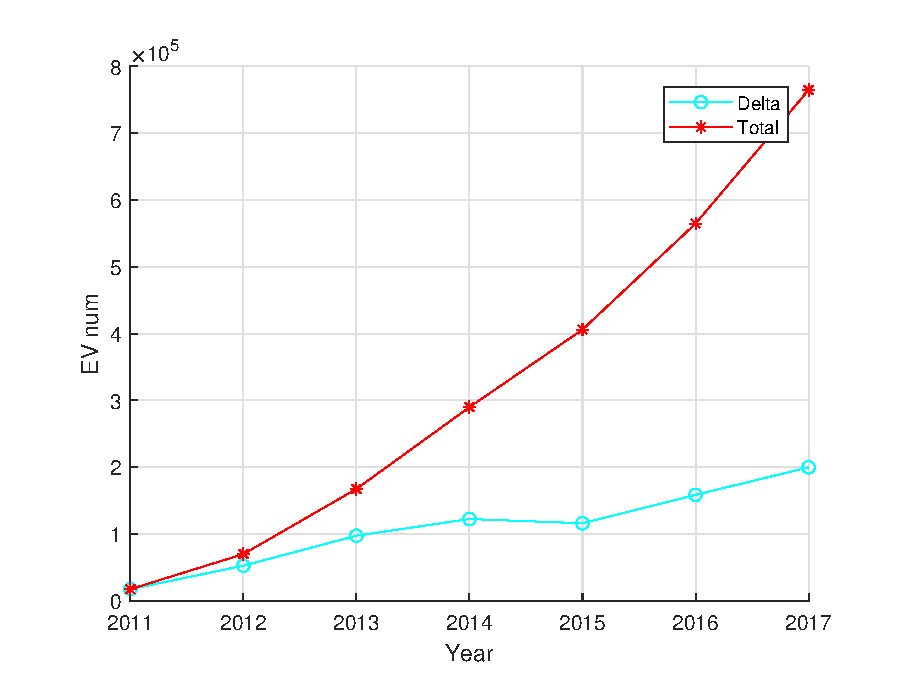
\includegraphics[width=14cm]{EVnum.eps}
\caption{EVnum} 
\end{figure}

\begin{figure}[htbp]
\small
\centering
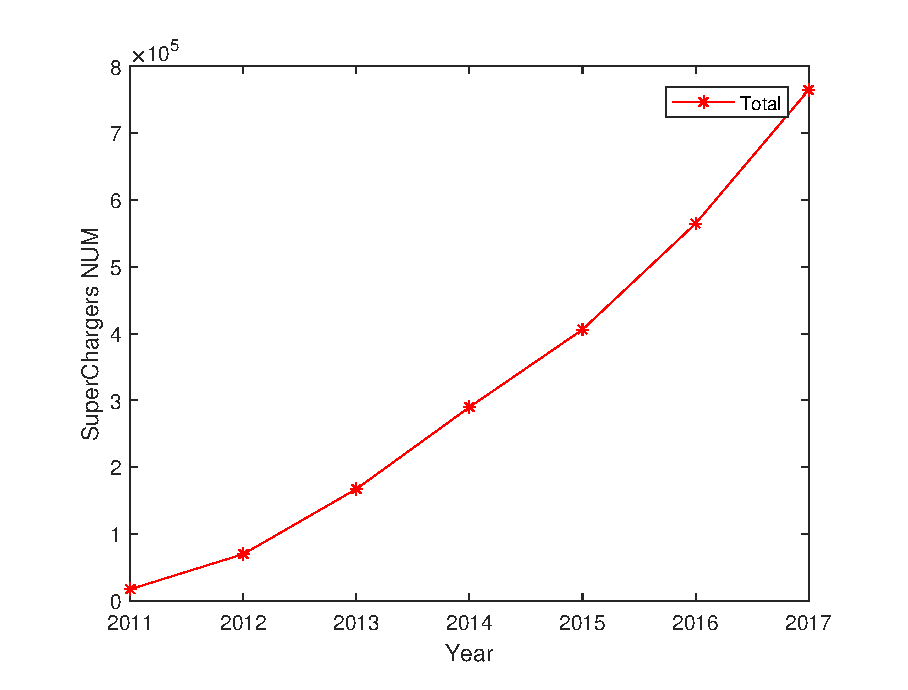
\includegraphics[width=14cm]{Superchargers.eps}
\caption{Superchargers} 
\end{figure}

\begin{figure}[htbp]
\small
\centering
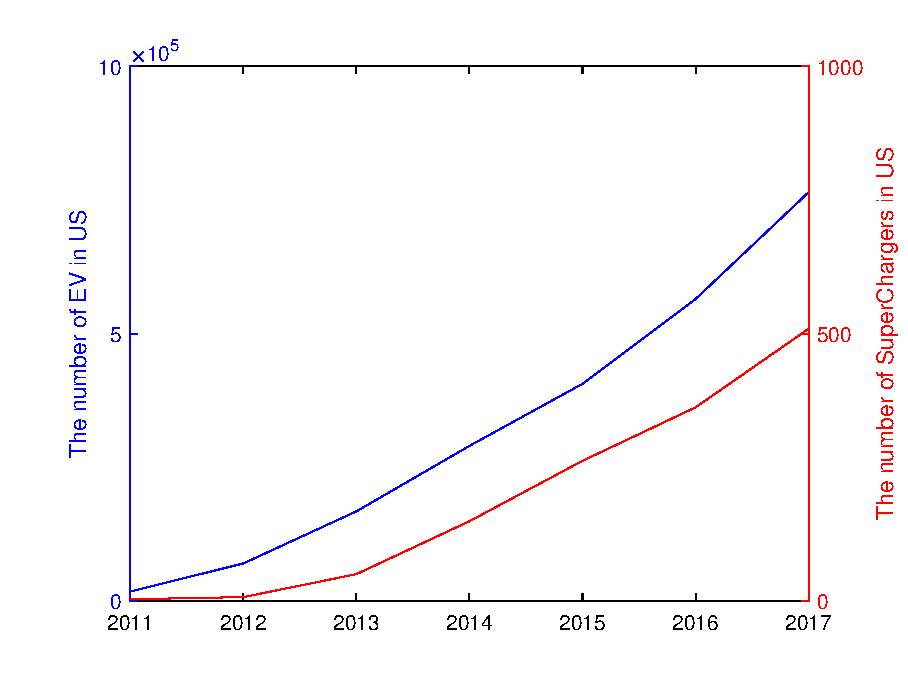
\includegraphics[width=14cm]{EVandChargers.eps}
\caption{EVandChargers} 
\end{figure}

\begin{figure}[htbp]
\small
\centering
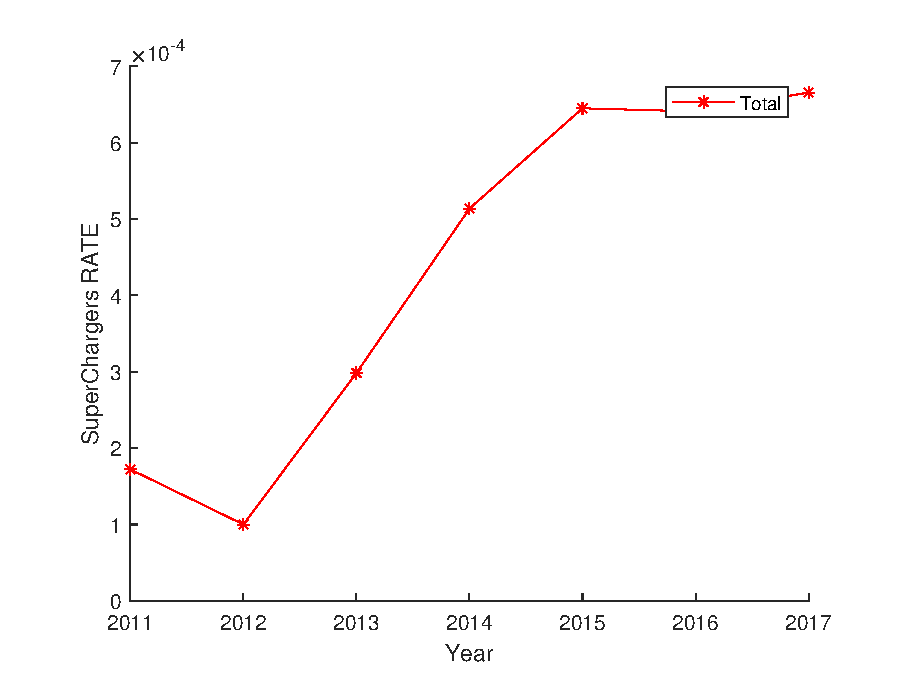
\includegraphics[width=14cm]{ChargerRate.eps}
\caption{ChargerRate} 
\end{figure}

\begin{table}[!htbp]
\centering
\begin{tabular}{|c|c|c|}
\hline
 &Super Charger&Destiny Charger \\
\hline
cost&1000k&50k\\
\hline
price& 1.8Yuan/kWh& 1.0Yuan/kWh\\
\hline
time& 30min~1.5h& 6h\\
\hline
method&FAST &SLOW \\
\hline
\end{tabular}
\caption{Compare}
\end{table}

\begin{figure}[htbp]
\small
\centering
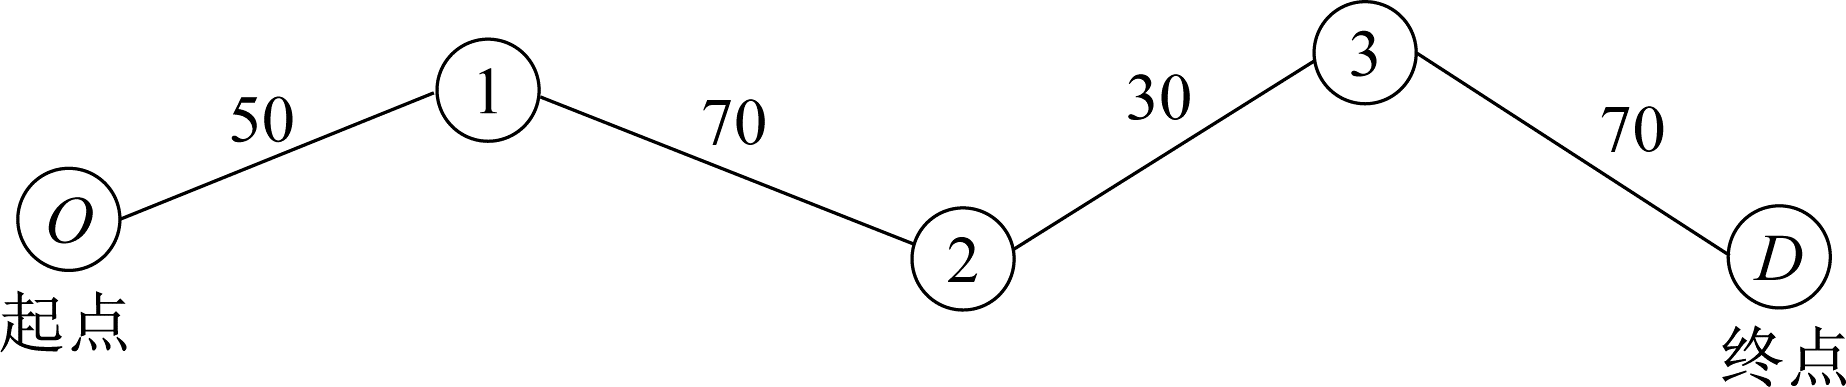
\includegraphics[width=12cm]{OD.png}
\caption{O-D Model} 
\end{figure}


\begin{figure}[htbp]
\small
\centering
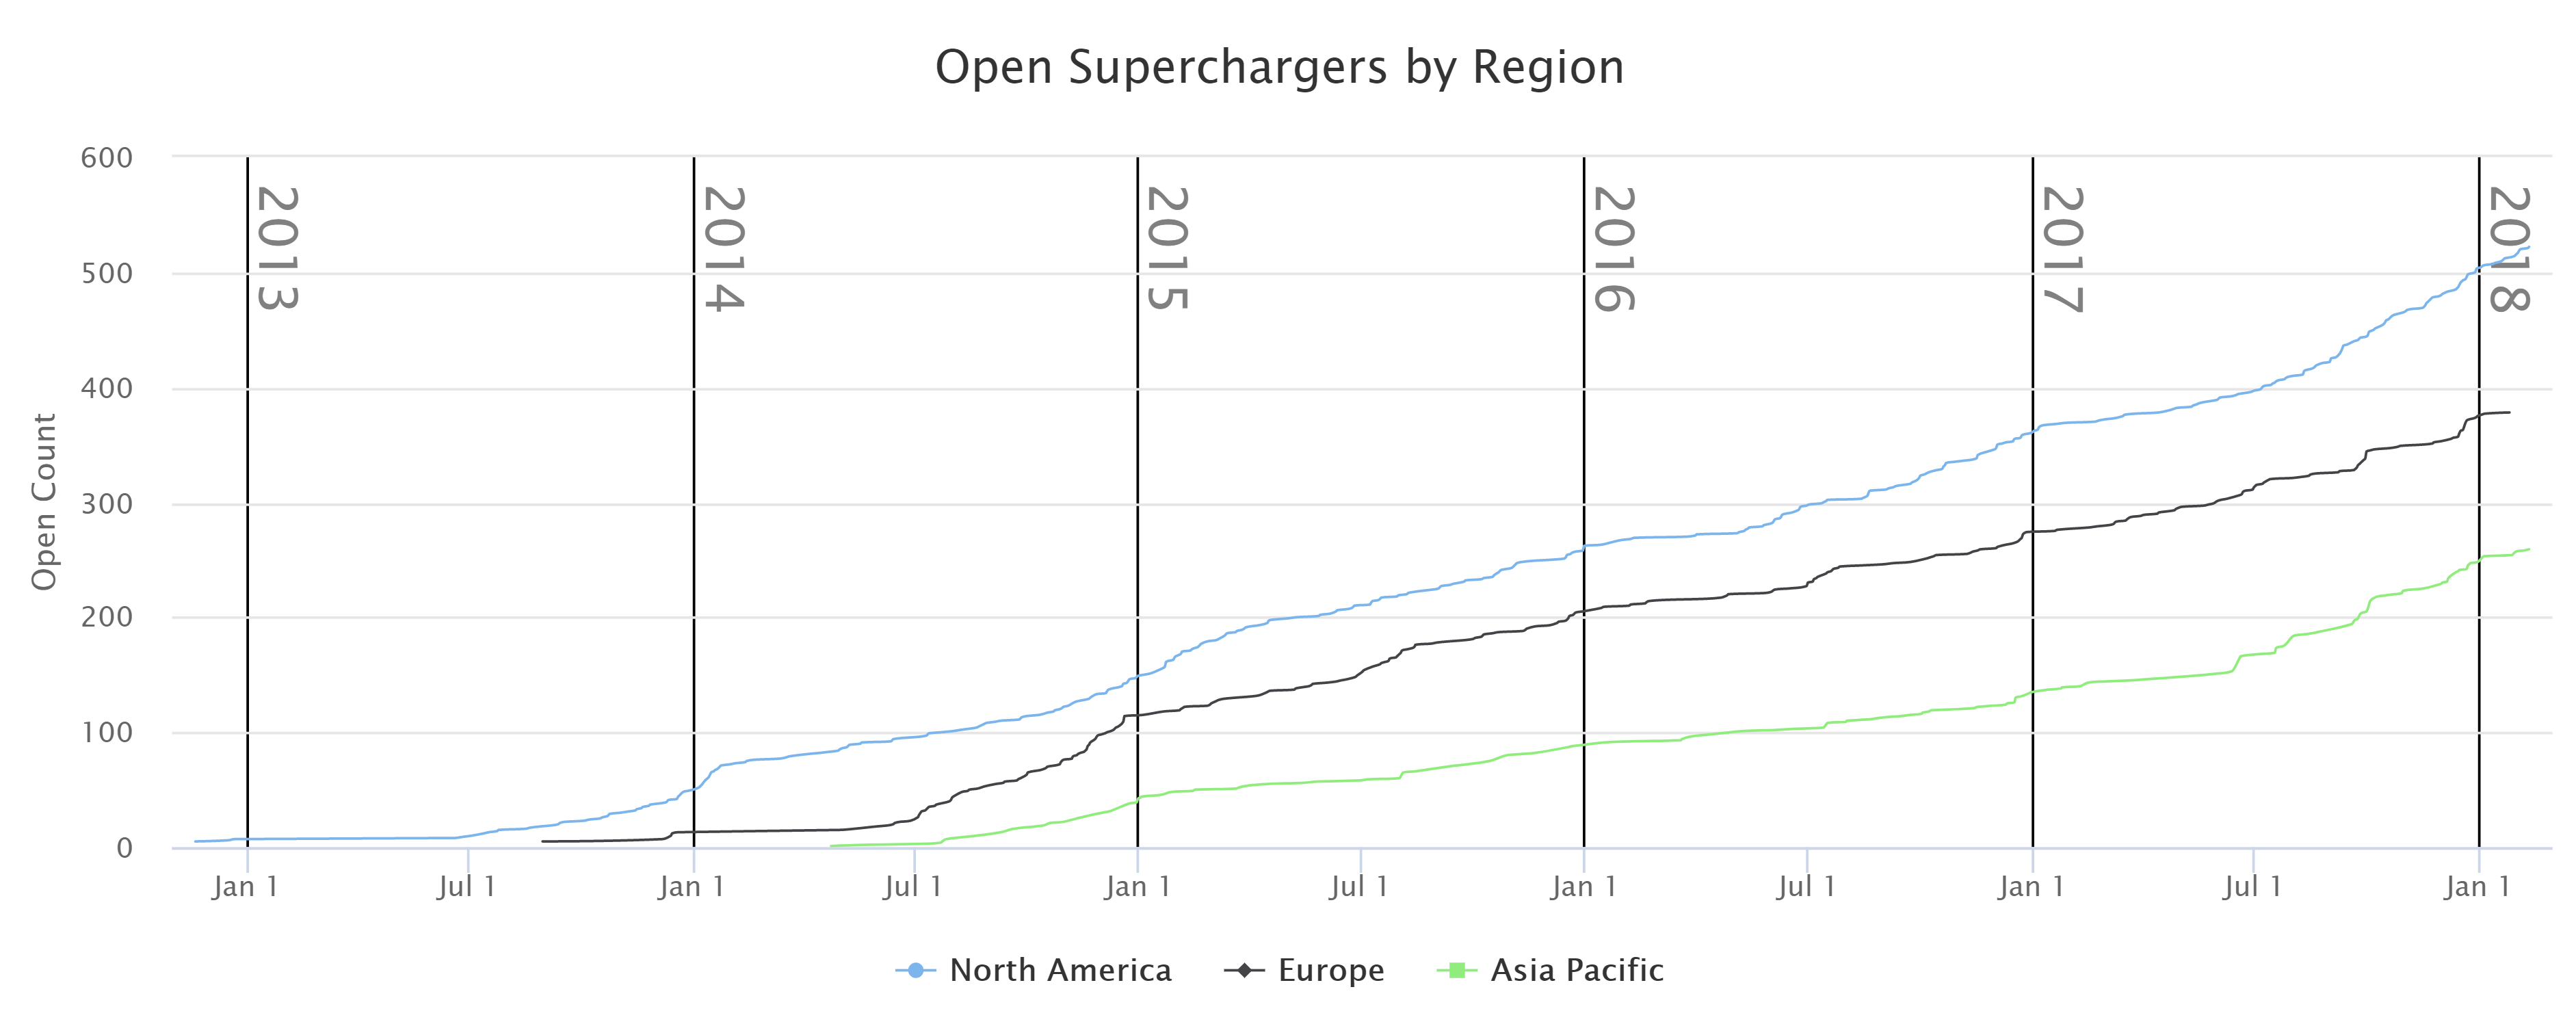
\includegraphics[width=16cm]{regions.png}
\caption{Open Superchargers By Regions} 
\end{figure}


\begin{figure}[htbp]
\small
\centering
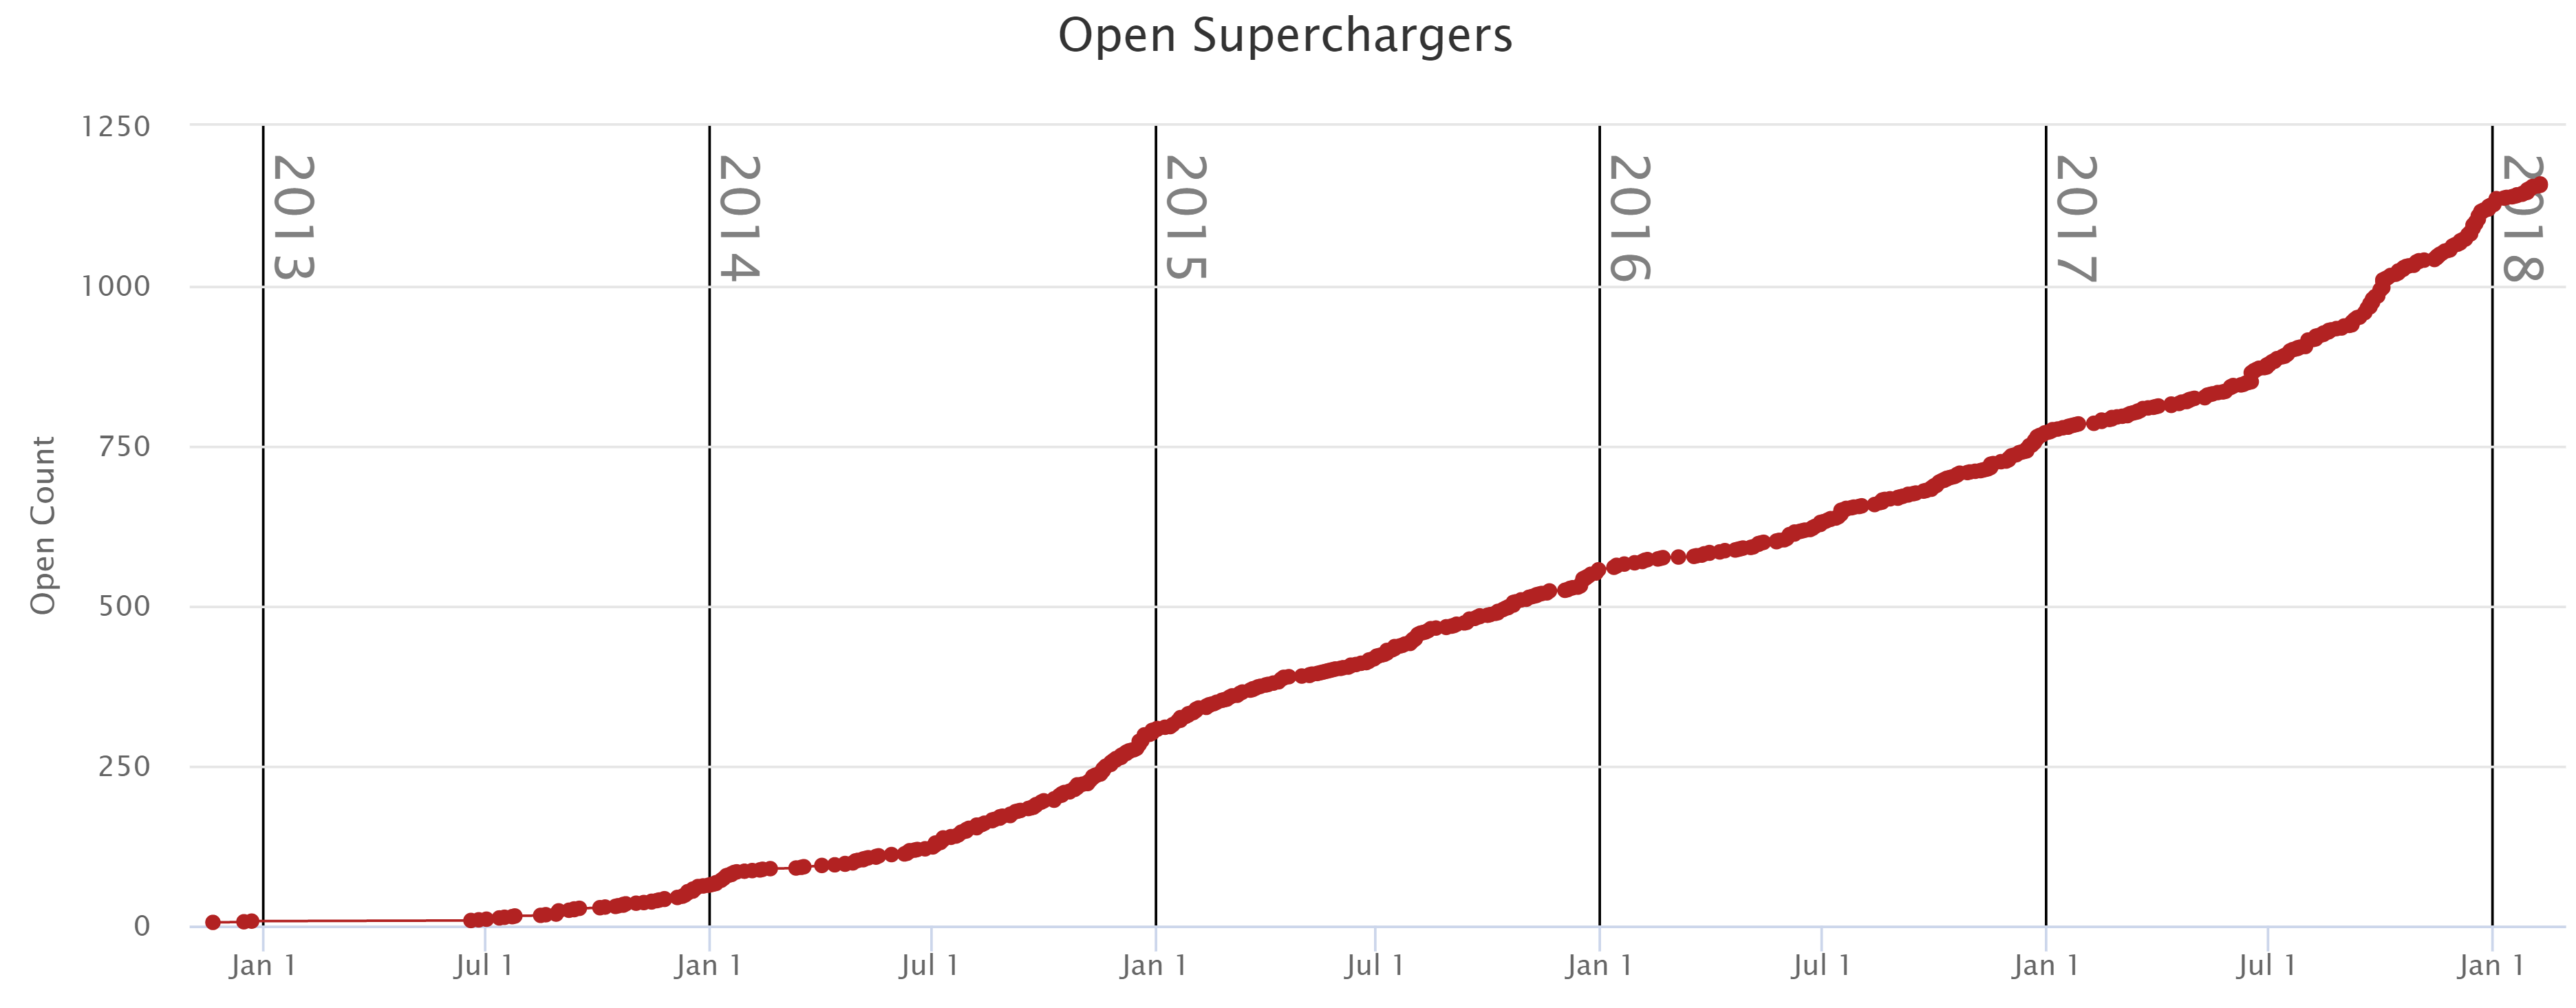
\includegraphics[width=16cm]{open.png}
\caption{Open Superchargers} 
\end{figure}


\begin{figure}[htbp]
\small
\centering
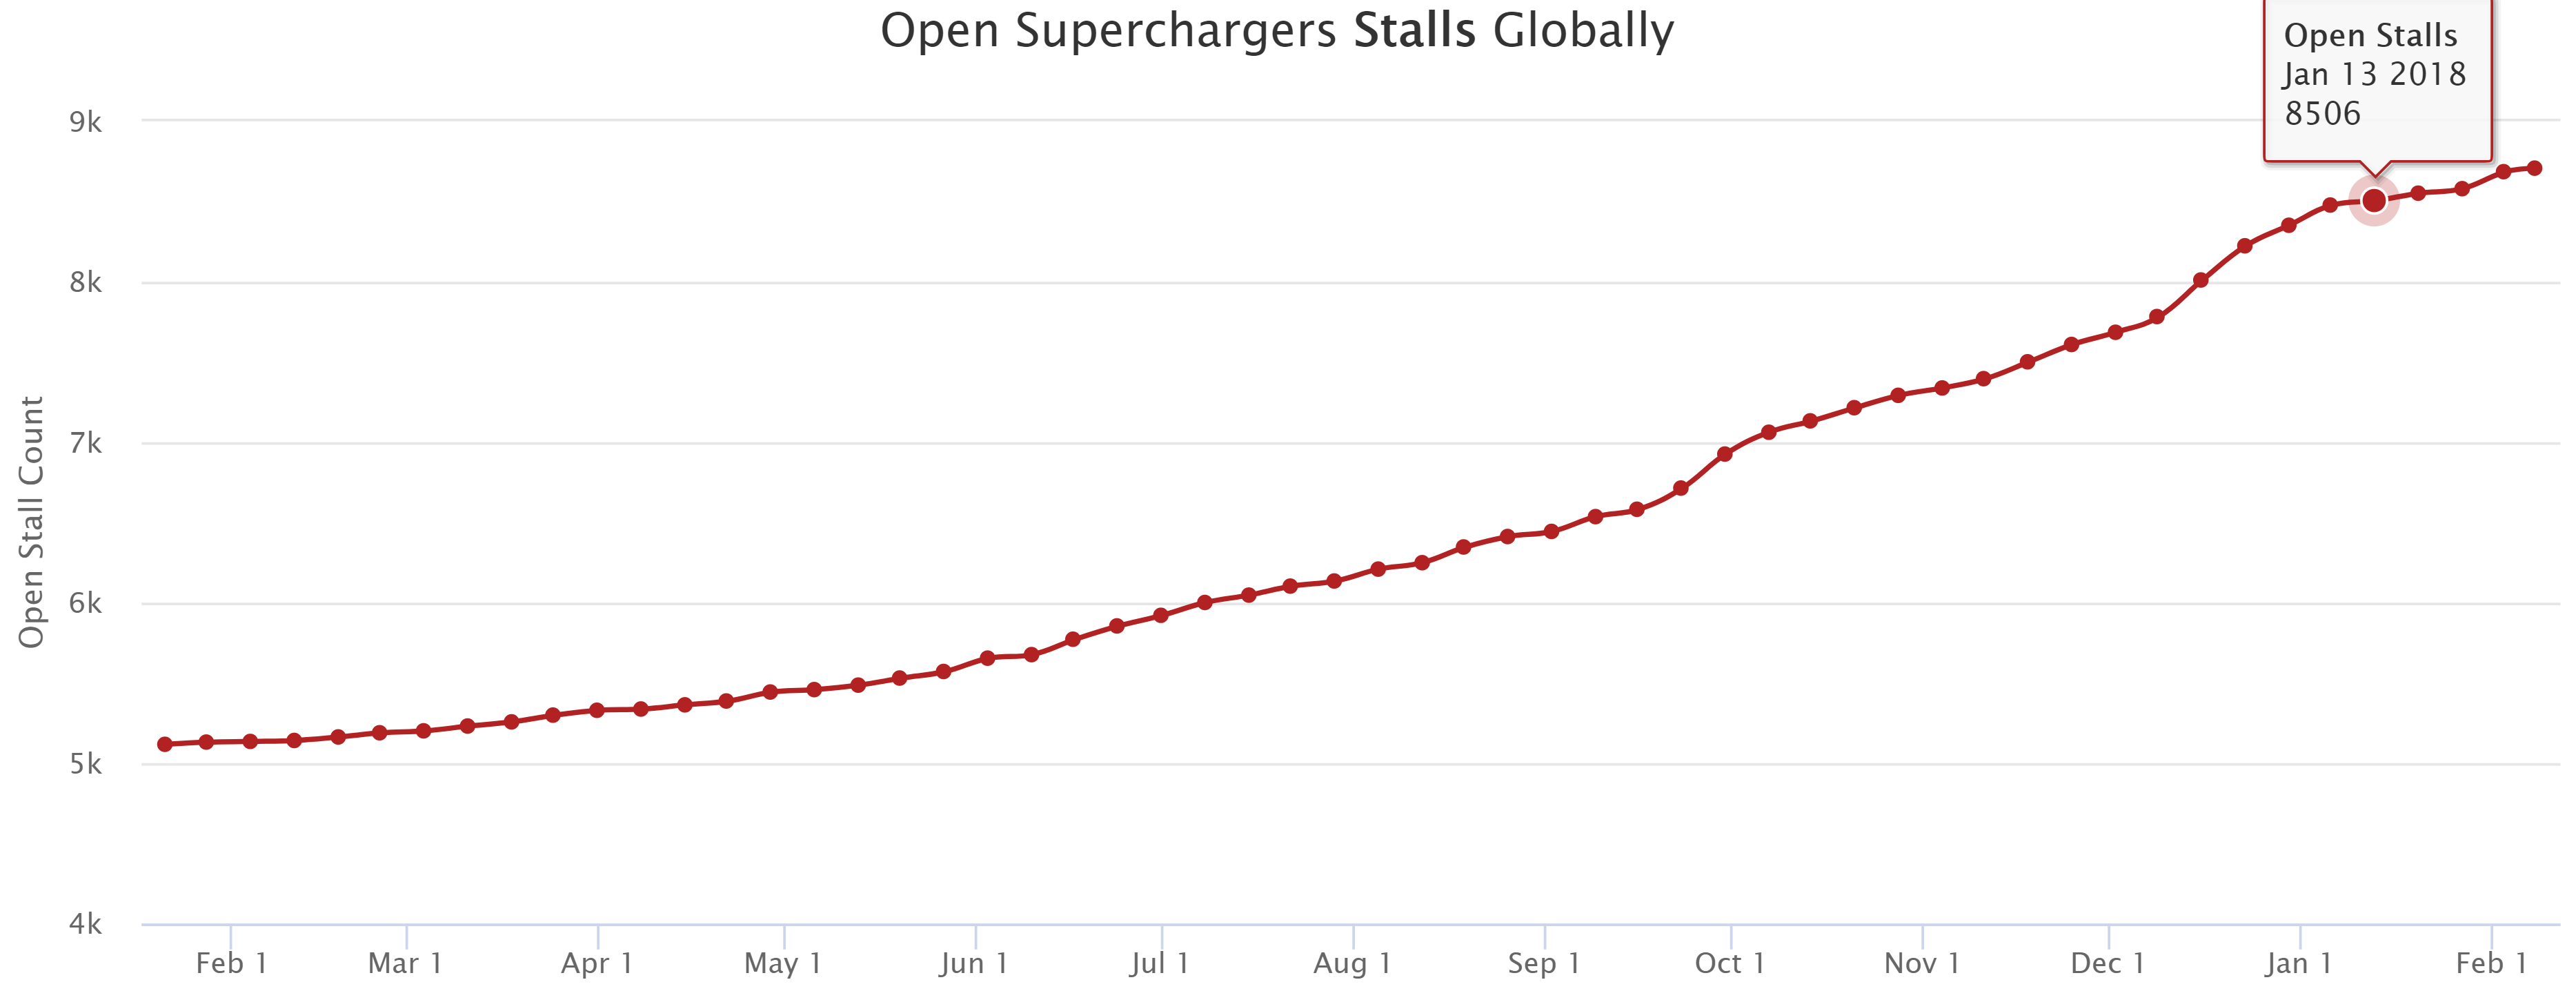
\includegraphics[width=16cm]{stall.png}
\caption{Open Superchargers Stall Globally} 
\end{figure}

\[
\min Z=\sum _{i\in S}C_{i}X_{i} + \sum _{i\in S}P_{i}Q_{i} + \sum _{i\in S}w_{i}Q\left( I_{i}\right)
\]

\[	
\sum _{m\in M}f_{m}R_{im} \leq Q\left( I_{i}\right)
\]

\[
i\rightarrow j\rightarrow k
\]


\section{Calculating and Simplifying the Model  }

\section{The Model Results}


\section{Validating the Model}


\section{Conclusions}


\section{A Summary}


\section{Evaluate of the Mode}

\section{Strengths and weaknesses}


\subsection{Strengths}
\begin{itemize}
\item \textbf{Applies widely}\\
This  system can be used for many types of airplanes, and it also
solves the interference during  the procedure of the boarding
airplane,as described above we can get to the  optimization
boarding time.We also know that all the service is automate.
\item \textbf{Improve the quality of the airport service}\\
Balancing the cost of the cost and the benefit, it will bring in
more convenient  for airport and passengers.It also saves many
human resources for the airline. 
\item \textbf{}
\end{itemize}

\begin{thebibliography}{99}
\bibitem{1} D.~E. KNUTH   The \TeX{}book  the American
Mathematical Society and Addison-Wesley
Publishing Company , 1984-1986.
\bibitem{2}Lamport, Leslie,  \LaTeX{}: `` A Document Preparation System '',
Addison-Wesley Publishing Company, 1986.
\bibitem{3}\url{https://supercharge.info/}
\bibitem{4}\url{https://insideevsforum.com/}
\end{thebibliography}

\begin{appendices}

\section{First appendix}

Here are simulation programmes we used in our model as follow.\\

\textbf{\textcolor[rgb]{0.98,0.00,0.00}{Input matlab source:}}
\lstinputlisting[language=Matlab]{./code/SuperChargeStation.m}

\textbf{\textcolor[rgb]{0.98,0.00,0.00}{Input matlab source:}}
\lstinputlisting[language=Matlab]{./code/EVusage.m}

Here is the Rate simulation:\\

\textbf{\textcolor[rgb]{0.98,0.00,0.00}{Input matlab source:}}
\lstinputlisting[language=Matlab]{./code/Rate.m}





\section{Second appendix}

some more text \textcolor[rgb]{0.00,0.90,0.00}{\textbf{Input C++ source:}}
\lstinputlisting[language=C++]{./code/mcmthesis-sudoku.cpp}

\end{appendices}
\end{document}




%% 
%% This work consists of these files mcmthesis.dtx,
%%                                   figures/ and
%%                                   code/,
%% and the derived files             mcmthesis.cls,
%%                                   mcmthesis-demo.tex,
%%                                   README,
%%                                   LICENSE,
%%                                   mcmthesis.pdf and
%%                                   mcmthesis-demo.pdf.
%%
%% End of file `mcmthesis-demo.tex'.
